\documentclass[12pt,aspectratio=169]{beamer}
\usetheme{metropolis}
\setbeamersize{text margin left=.5cm,text margin right=.5cm}
\usepackage[lf]{carlito}
\usepackage{siunitx}
\usepackage{tikz}
\usepackage{mathpazo}
\usepackage{bm}
\usepackage{mathtools}
\usepackage[ISO]{diffcoeff}
\diffdef{}{ op-symbol=\mathsf{d} }
\usepackage{xcolor,colortbl}

\setmonofont{Ubuntu Mono}
\setlength{\parskip}{0pt}
\renewcommand{\baselinestretch}{1}

\sisetup{
  inter-unit-product=\cdot,
  per-mode=symbol
}

\tikzset{
  >=latex
}

%\newcommand{\iii}{\hat{\bm\imath}}
%\newcommand{\jjj}{\hat{\bm\jmath}}
%\newcommand{\kkk}{\hat{\bm k}}


\title{Class 19A: Hall Effect}
\subtitle{Advanced Placement Physics C}
\author[TML]{Dr.\ Timothy Leung}
\institute{Olympiads School}
\date{Updated: Summer 2022}

\newcommand{\pic}[2]{
  \includegraphics[width=#1\textwidth]{#2}
}
\newcommand{\eq}[2]{
  \vspace{#1}{\Large
    \begin{displaymath}
      #2
    \end{displaymath}
  }
}
%\newcommand{\iii}{\ensuremath\hat{\bm{\imath}}}
%\newcommand{\jjj}{\ensuremath\hat{\bm{\jmath}}}
%\newcommand{\kkk}{\ensuremath\hat{\bm{k}}}
\newcommand{\iii}{\ensuremath\hat\imath}
\newcommand{\jjj}{\ensuremath\hat\jmath}
\newcommand{\kkk}{\ensuremath\hat k}



\begin{document}

\begin{frame}
  \maketitle
\end{frame}


\begin{frame}{Hall Effect}
  When a current $I$ flows through a conductor in a magnetic field
  $\vec B$, the magnetic field exerts a transverse (i.e.\ perpendicular to
  motion) magnetic force $\vec F_m$ on the moving charges which pushes them
  toward one side of the conductor.
  \begin{center}
    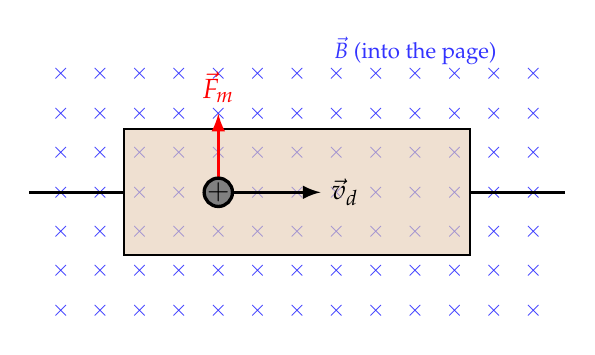
\begin{tikzpicture}
      \node at (4.5,3.8) {\textcolor{blue!80}{
          \footnotesize$\vec B$ (into the page)}
      };
      \foreach \x in {0,.5,...,6}{
        \foreach \y in {.5,1,...,3.5}{
          \node at (\x,\y) {\footnotesize\textcolor{blue!80}{$\times$}};
        }
      }
      \fill[brown!40,opacity=.6](.8,1.2) rectangle(5.2,2.8);
      \draw[thick](.8,1.2) rectangle(5.2,2.8);
      \draw[very thick](-.4,2)--(.8,2);
      \draw[very thick](5.2,2)--(6.4,2);

      \draw[->,very thick](2.18,2)--(3.3,2) node[right]{$\vec v_d$};
      \draw[->,very thick,red](2,2.18)--(2,3) node[above]{$\vec F_m$};
      \draw[very thick,fill=gray](2,2) circle(.18) node{$+$};
    \end{tikzpicture}
  \end{center}
  This is most evident in a \emph{thin}, \emph{flat} conductor as illustrated. 
\end{frame}



\begin{frame}{Magnetic Force}
  \begin{center}
    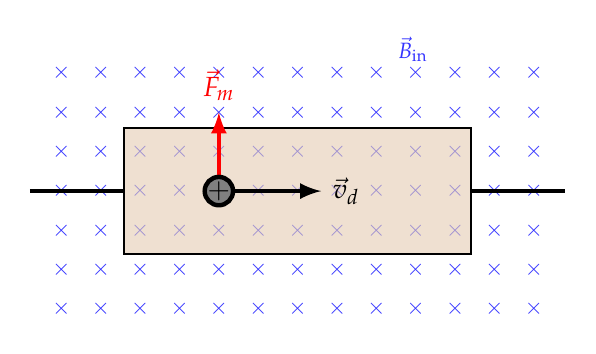
\begin{tikzpicture}
      \node at (4.5,3.8) {\textcolor{blue!80}{
          \footnotesize$\vec B_\text{in}$
        }
      };
      \foreach \x in {0,.5,...,6}{
        \foreach \y in {.5,1,...,3.5}{
          \node at (\x,\y) {\footnotesize\textcolor{blue!80}{$\times$}};
        }
      }
      \fill[brown!40,opacity=.6](.8,1.2) rectangle(5.2,2.8);
      \draw[thick](.8,1.2) rectangle(5.2,2.8);
      \draw[ultra thick](-.4,2)--(.8,2);
      \draw[ultra thick](5.2,2)--(6.4,2);

      \draw[->,ultra thick](2.18,2)--(3.3,2) node[right]{$\vec v_d$};
      \draw[->,ultra thick,red](2,2.18)--(2,3) node[above]{$\vec F_m$};
      \draw[ultra thick,fill=gray](2,2) circle(.18) node{$+$};
    \end{tikzpicture}
  \end{center}
  \vspace{-.1in}As the charges enter the magnetic field, $\vec F_m$ is directed
  toward the top:
  
  \eq{-.2in}{
    \vec F_m
    =e\textcolor{red}{\vec v_d}\times\vec B
    =\frac{e\textcolor{red}{\vec I}\times\vec B}{\textcolor{red}{neA}}
    =\frac{\vec I\times\vec B}{nA}
  }

  leading to a surplus of positive charges on the top edge of
  the conductor, and negative charges on the bottom.
\end{frame}



\begin{frame}[t]{Hall Voltage}
  \begin{center}
    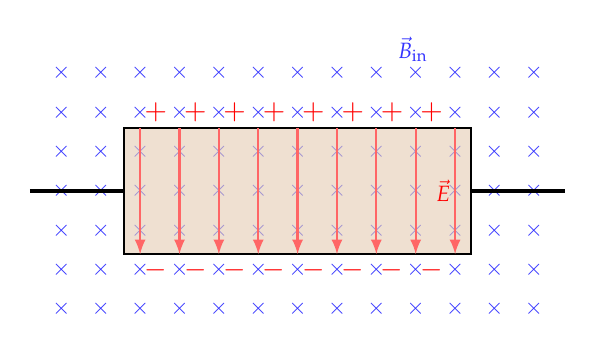
\begin{tikzpicture}
      \node at (4.5,3.8) {\textcolor{blue!80}{
          \footnotesize$\vec B_\text{in}$
        }
      };
      \foreach \x in {0,.5,...,6}{
        \foreach \y in {.5,1,...,3.5}{
          \node at (\x,\y) {\footnotesize\textcolor{blue!80}{$\times$}};
        }
      }
      \fill[brown!40,opacity=.6](.8,1.2) rectangle(5.2,2.8);
      \draw[thick](.8,1.2) rectangle(5.2,2.8);
      \draw[ultra thick](-.4,2)--(.8,2);
      \draw[ultra thick](5.2,2)--(6.4,2);

      \foreach \x in {1.2,1.7,...,5}{ \node at (\x,1){\textcolor{red}{$-$}};}
      \foreach \x in {1.2,1.7,...,5}{ \node at (\x,3){\textcolor{red}{$+$}};}
      \foreach \x in {1,1.5,...,5}{
        \draw[thick,->,red!60] (\x,2.8)--(\x,1.2);
      }
      \node at (4.85,2) {\textcolor{red}{\footnotesize$\vec E$}};
    \end{tikzpicture}
  \end{center}
  The charge imbalance on the conductor creates an electric field $\vec E$,
  pointing toward the bottom, and therefore a voltage across two sides of the
  conductor (width $W$), called the \textbf{Hall voltage}:

  \eq{-.25in}{
    V_H=EW
  }
\end{frame}



\begin{frame}{Balancing Electrostatic \& Magnetic Forces}
  \begin{center}
    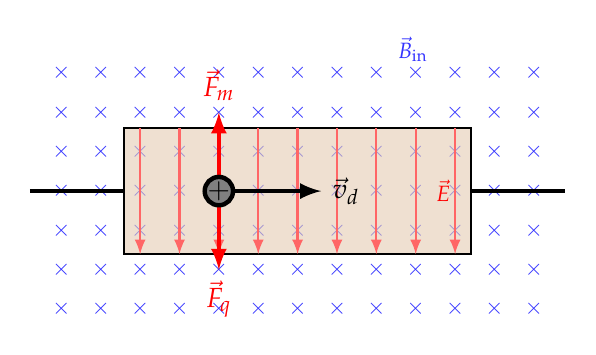
\begin{tikzpicture}
      \node at (4.5,3.8) {\textcolor{blue!80}{
          \footnotesize$\vec B_\text{in}$
        }
      };
      \foreach \x in {0,.5,...,6}{
        \foreach \y in {.5,1,...,3.5}{
          \node at (\x,\y) {\footnotesize\textcolor{blue!80}{$\times$}};
        }
      }
      \fill[brown!40,opacity=.6](.8,1.2) rectangle(5.2,2.8);
      \draw[thick](.8,1.2) rectangle(5.2,2.8);
      \draw[ultra thick](-.4,2)--(.8,2);
      \draw[ultra thick](5.2,2)--(6.4,2);

      \foreach \x in {1,1.5,...,5}{
        \draw[thick,->,red!60] (\x,2.8)--(\x,1.2);
      }
      \node at (4.85,2) {\textcolor{red}{\footnotesize$\vec E$}};
      
      \draw[->,ultra thick](2.18,2)--(3.3,2) node[right]{$\vec v_d$};
      \draw[->,ultra thick,red](2,2.18)--(2,3) node[above]{$\vec F_m$};
      \draw[->,ultra thick,red](2,1.82)--(2,1) node[below]{$\vec F_q$};
      \draw[ultra thick,fill=gray](2,2) circle(.18) node{$+$};
    \end{tikzpicture}
  \end{center}
  Subsequently, charge carriers entering the magnetic field will experience
  both a magnetic force and an electrostatic force. At equilibrium, the two
  forces are balanced:

  \eq{-.3in}{
    \vec F_m+\vec F_q=\vec 0
  }
\end{frame}



\begin{frame}{Calculating Hall Voltage}
  The electrostatic force on the charge carrier can be expressed in terms of
  the Hall voltage $V_H$ across the two sides of the plate:

  \eq{-.15in}{
    F_q=eE=\frac{eV_H}W
  }
  
  Equating the magnitudes of electrostatic and magnetic forces, we can solve
  for the Hall voltage:

  \eq{-.2in}{
    F_m=F_q\quad\rightarrow\quad
    \frac{IB}{nA}=\frac{eV_H}W
  }
\end{frame}


\begin{frame}{Hall Voltage}
  Cancelling terms and noting that the thickness of the conductor is

  \eq{-.2in}{
    d=\frac AW
  }

  we find the expression for the Hall voltage $V_H$:

  \eq{-.1in}{
    \boxed{V_H=\frac{IB}{ned}}
  }
\end{frame}



\begin{frame}{Hall Probe}
  Large magnetic fields ($\sim$ \SI1\tesla) is often measured using a
  \textbf{Hall probe}. A thin film Hall probe is placed in the magnetic field
  and the transverse voltage (usually measured in on the order of
  \SI{e-6}\volt) is measured.

  \begin{center}
    \pic{.3}{hallp}
  \end{center}
  The polarity of the Hall voltage for a copper probe shows that electrons
  (negative charge) are the charge carriers.
\end{frame}
\end{document}
